\cotefile{37}

\scanpage{87}
\mspage{539}

\noindent\qquad 3.8. Quasi-homéomorphismes et images réciproques de faisceaux\dotfill

\noindent\qquad 3.9. Faisceaux d'espaces pseudo-discrets\dotfill

\noindent\quad \S\ 4. Espaces annelés\dotfill

\noindent\qquad 4.1. Espaces annelés , $A$-Modules , $A$-Algèbres\dotfill

\noindent\qquad 4.2. Image directe d'un $A$-Module\dotfill

\noindent\qquad 4.3. Image réciproque d'un $B$-Module\dotfill

\noindent\qquad 4.4. Relations entre images directes et images réciproques\dotfill

\noindent\qquad 4.5.Immersions ouvertes et morphismes représentables par des immersions ouvertes \dotfill

\noindent\quad \S\ 5. Faisceaux quasi-cohérents et faisceaux cohérents\dotfill

\noindent\qquad 5.1. Faisceaux quasi-cohérents\dotfill

\noindent\qquad 5.2. Faisceaux de type fini\dotfill

\noindent\qquad 5.3. Faisceaux cohérents\dotfill

\noindent\qquad 5.4. Faisceaux localement libres\dotfill

\noindent\qquad 5.5. Modules localement libres sur un espace localement annelé\dotfill

\noindent\qquad 5.6. Groupe de Picard\dotfill

\noindent\qquad 5.7. Morphismes plats d'espaces annelés\dotfill

\noindent\quad \S\ 6. Compléments d'algèbre commutative .

\noindent\qquad 6.1. Limites inductives d'anneaux\dotfill

\noindent\qquad 6.2. Identification du module $M_f$ à une limite \deleted{\unsure{project|projecti}} inductive\dotfill

\noindent\qquad 6.3. Propriétés de finitude\dotfill

\noindent\qquad 6.4. Critères pour qu'un anneau soit noethérien\dotfill

\noindent\qquad 6.5. Anneaux normaux et ferm\unsure{\deleted{t}e\deleted{e}t|\deleted{e}t\deleted{t}e}ure intégrale\dotfill

\noindent\qquad 6.6. Compléments sur la platitude\dotfill

\noindent\qquad 6.7. Compléments sur\deleted{l} les modules projectifs\dotfill

\noindent\qquad 6.8. Existence d'extensions plates d'anneaux locaux\dotfill

\noindent\quad \deleted{\S\ \unsure{7.}}

\noindent\quad \S\ 7. Compléments d'algèbre topologique\dotfill

\noindent\qquad 7.1. Anneaux admissibles\dotfill

\noindent\qquad 7.2. Anneaux adiques et limites projectives\dotfill

\noindent\qquad 7.3. Anneaux préadiques noethériens\dotfill

\noindent\qquad 7.4. Modules quasi-finis sur les anneaux locaux\dotfill

\noindent\qquad \deleted{7\unsure{.}} 7.5. Anneaux de séries formelles restreintes\dotfill

\noindent\qquad 7.6. Anneaux complets de fractions\dotfill

% archive sheet number: 86

\scanpage{88}
\mspage{540}

\noindent\qquad 7.7. Produits tensoriels complétés\dotfill

\noindent\qquad 7.8. Topologies sur les modules d'homomorphismes\dotfill

\noindent CHAPITRE I .- Le langage des schémas\dotfill

\noindent\quad Sommaire\dotfill

\noindent\quad \S\ 1. Schémas affines\dotfill

\noindent\qquad 1.1. Le spectre premier d'un anneau\dotfill

\noindent\qquad 1.2. Propriétés fonctorielles des spectres premiers d'anneaux\dotfill

\noindent\qquad 1.3. Faisceau associé à un module\dotfill

\noindent\qquad 1.4. Faisceaux quasi-cohérents sur un spectre premier\dotfill

\noindent\qquad 1.5. Faisceaux cohérents sur un spectre premier\dotfill

\noindent\qquad \deleted{S}1.6.Schémas affines et morphismes d'espaces localement annelés dans des schémas affines\dotfill

\noindent\qquad 1.7.Images directes et images réciproques de faisceaux quasi-cohérents par des morphismes de schémas affines\dotfill

\noindent\quad \S\ 2. Schémas et morphismes de schémas\dotfill

\noindent\qquad 2.1. Définition des schémas\dotfill

\noindent\qquad 2.2. Faisceaux quasi-cohérents sur un schéma\dotfill

\noindent\qquad 2.3. Morph\deleted{\unsure{u|n}}ismes de schémas\dotfill

\noindent\qquad 2.4. Recollement de schémas\dotfill

\noindent\qquad 2.5. Schémas locaux\dotfill

\noindent\qquad 2.6. Schémas au-dessus d'un schéma\dotfill

\noindent\qquad 2.7. Schémas noethériens et schémas localement noethériens\dotfill

\noindent\qquad 2.8. Schémas artiniens\dotfill

\noindent\quad \S\ 3. Produit et somme de schémas. Changement de base\dotfill

\noindent\qquad 3.1. Somme de schémas\dotfill

\noindent\qquad 3.2. Produit de schémas\dotfill

\noindent\qquad 3.3. Produit tensoriel de Modules quasi-cohérents sur un produit de schémas\dotfill

\noindent\qquad 3.4. Changements de base ; fibres\dotfill

\noindent\qquad 3.5. Points d'un schéma à valeurs dans un schéma ; points géométriques\dotfill

\noindent\qquad 3.6. Morphismes surjectifs\dotfill

\noindent\qquad 3.7. Morphismes radiciels\dotfill

% archive sheet number: 87

\scanpage{89}
\mspage{\handwritten{542} \unsure{\deleted{\unsure{5|3|B|6}}|\deleted{\unsure{X|3}}\unsure{5|B|6}}}

\noindent § 7. Ensembles constructibles dans les schémas\dotfill

7.1. Morphismes de présentation finie et ensembles constructibles\dotfill

7.2. Ensembles pro-constructibles et ind-constructibles.

7.3. Application aux morphismes générisants\dotfill

\noindent § 8. Applications rationnelles \dotfill

8.1. Applications rationnelles et fonctions rationnelles

8.2. Domaine de définition d'une application rationnelle

8.3. Faisceau des fonctions rationnelles\dotfill

8.4. Faisceaux de torsion et faisceaux sans torsion\dotfill

8.5. Critères de séparation d'un schéma intègre\dotfill

\noindent § 9. Foncteurs représentables élémentaires dans la théorie des schémas : Schémas relativement affines , fibrés vectoriels , fibrés projectifs et grassmanniennes..

9.1. Morphismes affines et spectres d'Algèbres quasi-cohérentes\dotfill

9.2. Faisceaux quasi-cohérents sur un $S$-schéma affine sur $S$\dotfill

9.3. Application aux changelents de base pour les images directes de Modules quasi-cohérents\dotfill

9.4. Fibré vectoriel associé à un faisceau de modules\dotfill

9.5. Schémas en ensembles algébriques\dotfill

9.6. Schémas en groupes linéaires\dotfill

9.7. Grassmanniennes d'un Module\dotfill

9.8. Morphismes de Plücker et de Segre\dotfill

9.9. F\deleted{\unsure{u|o|i}}ibrés en drapeaux\dotfill

9.10.Fibrés en variétés de Stiefel\dotfill

\noindent § 10. Schémas formels\dotfill

10.1. Schémas formels affines\dotfill

10.2. Morphismes de schémas form\unsure{\deleted{l}e|\deleted{e}l}\unsure{\deleted{e}l|\deleted{s}l|\deleted{l}e|\deleted{l}s}s affines\dotfill

10.3. Idéaux de définition d'un schéma formel affine\dotfill

10.4. Schémas formels et morphismes de schémas formels\dotfill

10.5. Idéaux de définition des schéma\unsure{\deleted{q}s|\deleted{s}q} formels\dotfill

10.6. Schémas formels comme limite inductives de schémas

10.7. Produit de schémas formels\dotfill

10.8. Complété formel d'un schéma le long d'un sous-schéma\dotfill
% archive sheet number: 88

\scanpage{90}
\begin{center}-\qquad -\end{center}

Spectre formel d'un anneau admissible : I,10.1.2 .

Spectre d'une $O_S$-Algèbre : I,9.1.8.

Stabilisateur d'une section d'un Module localement libre de rang fini : I,9.6.6.

Support d'un faisceau de groupes : \deleted{\unsure{0,1.6|0,1.1}} 0,3.1.6 .

Support d'une section d'un faisceau de groupes : 0,3.1.6 .

Système fondamental d'idéaux (de sous-modules) ouverts : 0,7.1.1.

Système fondamental d'Idéaux de définition : I,10.3.6 et 10.5.1.

Système inductif dans une catégorie : 0,1.1.12 .

Système inductif adique de schémas : I,10.12.2 .

Système projectif dans une catégorie : 0,1.1.9 .

Topologie canonique d'un anneau semi-local : 0,7.3.1.

Topologie constructible sur un schéma : \deleted{I,6} I,7.2.11 .

Topologie déduite de celle de $A$ sur un $A$-module : 0,7.1.1.

Topologie $J$-adique , topologie $J$-préadique : 0,7.1.9 et 7.2.3 .

Topologie spectrale : I,1.1.2 .

Topologie produit tensoriel : 0,7.7.2 .

Trait : I,5.5.1 .

Très dense (partie) : 0,2.6.3 .

Trivial ($O_X$-Module inversible) : I,2.5.7 .

Type fini ($O_X$-Module de) : 0,5.2.1.

Ultra-schéma : I,App.1.5 .

Valeur\deleted{ d'une section} en un point d'une section d'un $O_X$-Module sur un espace localement annelé : 0,4.1.9 .
% archive sheet number: 89

\scanpage{91}
\mspage{543}

10.9. Prolongement d'un morphisme aux complétés\dotfill

10.10. Modules de présentation finie sur les schémas formels affines adiques\dotfill

10.11.Modules de présentation finie sur les schémas formels adiques\dotfill

10.12. Morphismes adiques de schémas formels\dotfill

10.13. Morphismes de type fini\dotfill

10.14. Sous-schémas fermés des schémas formels\dotfill

10.15. Schémas formels séparés\dotfill
\margin{\figure{\makebox[0pt][l]{\hspace{0.1cm}\raisebox{1.1cm}[0pt][0pt]{\makebox[1.79cm]{\handwritten{\inserted{\shortstack{Morphismes\\\unsure{affines|finis}}}}}}}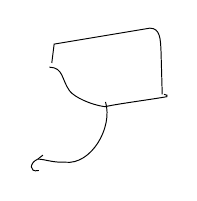
\begin{tikzpicture}[x=0.75cm,y=0.75cm]
\draw[line width=0.35pt] (0.12,-0.62) -- (0.16,-0.30) -- (1.78,-0.03)
  .. controls (1.96,-0.03) and (1.96,-0.22) .. (1.97,-0.43) -- (1.99,-1.15);
\draw[line width=0.35pt] (0.08,-0.69)
  .. controls (0.32,-0.70) and (0.28,-0.89) .. (0.42,-1.09)
  .. controls (0.50,-1.20) and (0.79,-1.33) .. (1.02,-1.36)
  .. controls (1.24,-1.31) and (1.79,-1.24) .. (2.07,-1.19)
  .. controls (2.10,-1.18) and (2.06,-1.15) .. (2.02,-1.15);
\draw[line width=0.35pt] (1.03,-1.28)
  .. controls (1.16,-1.72) and (0.78,-2.35) .. (0.35,-2.30)
  .. controls (0.12,-2.31) and (-0.02,-2.24) .. (-0.12,-2.25);
\draw[line width=0.35pt] (-0.12,-2.25)
  .. controls (-0.25,-2.30) and (-0.28,-2.48) .. (-0.10,-2.44);
\draw[line width=0.35pt] (-0.12,-2.25) -- (-0.03,-2.18);
\end{tikzpicture}}}

APPENDICE .- Ultraschémas et espaces algébriques de Serre\dotfill

App.1. Spectres maximaux et ultraschémas\dotfill

App.2. Espaces algébriques de Serre\dotfill

BIBLIOGRAPHIE\dotfill

INDEX DES NOTATIONS\dotfill

INDEX TERMINOLOGIQUE\dotfill

\begin{center}\rule{2cm}{0.4pt}\end{center}
% archive sheet number: 90

\scanpage{92}
\begin{center}-\qquad -\end{center}

$S$-schéma localement quasi-fini sur $S$ : I,6.11.3 .

- quasi-compact sur $S$ : I,6.1.1 .

- quasi-séparé sur $S$ : I,6.1.3 .

- quasi-fini sur $S$ : \deleted{\unsure{6,|I,}} I,6.11.3 .

- séparé sur $S$ : I,5.2.1 .

\deleted{\unsure{S-dominantes|S-dominants}} Schéma formel : I,10.4.2 .

- adique : I,10.4.2 .

- affine : I,10.1.2 .

- localement noethérien : I,10.4.2 .

- noethérien : I,10.4.2 .

- séparé : I,10.15.1 .

$A$-schéma formel , schéma formel sur $A$ ($A$ anneau admissible) :I,10.4.7

$S$-schéma formel , schéma formel sur $S$ ($S$ schéma formel) : I,10.4.7.

$S$-schéma formel de type fini sur $S$ : I,10.13.3 .

$S$-schéma formel séparé sur $S$ : I,10.15.1 .

Section d'un faisceau au-dessus d'un ouvert : 0,3.1.6 .

Section unité de $O_X$ : 0,4.1.1 .

$S$-section d'un $S$-objet : 0,1.1.11 .

$S$-section\deleted{s} d'un $S$-schéma : I,2.6.5 et 5.1.4 .

$S$-section universelle d'un $S$-objet : 0,1.4.9 .

$S$-section rationnelle d'un $S$-schéma : I,8.1.2 .

Série formelle restreinte : 0,7.5.1 .

Somme de schémas : \deleted{\unsure{I,3.1.1}} I,3.1.

Somme amalgamée d'objets de \uline{$C$} : 0,1.2.16 .

Sous-$O_X$-Algèbre engendrée par un sous-Module : 0,4.1.3 .

Sous-catégorie , sous-catégorie \deleted{\illegible{1}} pleine : 0,1.1.5 .

Sous-espace annelé d'un espace annelé : I,4.2.5 .

\deleted{So\unsure{u|y}s-} Sous-foncteur : 0,1.7.1 .

Sous-schéma : I,4.1.2 .

Sous-schéma associé à une immersion : I,4.2.1 .

Sous-schéma fermé : I,4.\unsure{\deleted{2}1|\deleted{1}2}.2 .

Sous-schéma fermé défini par un Idéal quasi-cohérent : I,4.1.1.

Sous-schéma des coïncidences de deux morphismes : I,5.1.5 .

Sous-schéma majoré par un sous-schéma : I,4.3.8 .

Sous-schéma schématiquement dense : I,5.4.2 .

Sous-schéma formel fermé : I,10.14.2 .

Spécialisation : 0,2.1.1 .

Spectre (ou spec\unsure{\deleted{r}t\deleted{t}r|\deleted{t}r\deleted{r}t}e premier) d'un anneau : I,1.1.1.

Spectre maximal d'un anneau de Jacobson : I,App.1.3 .
% archive sheet number: 91

\scanpage{93}
\noindent\hfill\handwritten{\unsure{27|22}.8.1967.}\\

\noindent Cher Dieudonné,\\

Tu as bien fait de tiquer sur la généralisation que je suggérai de EGA I 10.10.5. Je pense que l'analogue nonnoethérien de l'équivalence de a) et c) doit sortir sans mal, mais en tous cas ces conditions ne son\unsure{t} pas impliquées par b). P\unsure{q|g|\deleted{q}o|\deleted{g}o}ur le voir, soit $A=B\handwritten{[[}T\handwritten{]]}$ , et définissons
\[
M_n\handwritten{\unsure{(}}=A_n/J_{\deleted{\unsure{p|y}}n}\ ,\quad\text{où}\quad A_n=B\handwritten{[}T\handwritten{]}/(T^{n+1})\ ,\quad J_n=(X_o,X_1T,..,X_nT^n\handwritten{\unsure{)}}
\]
en choisissant l'anneau $B$ et les $X_n\handwritten{\in}B$ de telle façon que les générateurs écrits de $J_n$ soient en nombre minimal. IL suffit pour ceci de prendre pour $B$ un anneau de polynômes
\[
B=k\handwritten{[}(X_i)_{1\handwritten{\geq}0}\handwritten{]}\ ,
\]
on vérifie en effet que les générateurs écrits donnent alors dans $J_n/TJ_n$ des éléments linéairement indépendants sur $\deleted{B/T}\ A_o=A/TA=B$ . En effet, si les $a_i\handwritten{\in}B$ $(0\handwritten{\leq}i\handwritten{\leq}n)$ sont tels que
\[
a_oX_o+\ldots+\deleted{\unsure{t}}a_nX_nT^n=F_oX_oT+\ldots+F_nX_nT^{n+1}\ ,
\]
où les $F_n$ sont dans $B\handwritten{[}T\handwritten{]}=A\handwritten{[}T,(X_i)\handwritten{]}$ , on voit pour tout $i$, $0\handwritten{\leq}i\handwritten{\leq}n$, divisant par l'idéal engendré par les $X_j$ avec $j\handwritten{\ne}i$ , qu'on a une relatio\unsure{n}
\[
a_iX_iT^i=F'_iX_iT^{i+1}\quad\text{dans}\quad k\handwritten{[}X_i,T\handwritten{]},
\]
où $F'_i$ est l'image de $F_i$ . Comme $X_i$ et $T$ sont des éléments réguliers de cet anneau, on en conclut que
\[
a_i=F'_i\,T\quad\text{dans}\quad k\handwritten{[}X_i,T\handwritten{]}\ ,
\]
d'où évidemment $a_i=0$ , cqfd.

Je suggère donc de rédiger la nouvelle proposition 10.10.5 en disant qu'on a deux conditions équivalentes \deleted{\unsure{en|et}} impliquant une troisième condition, et que cette dernière équivaut aux deux autres dans le cas noethérien. Il serait peut-être utile de donner aussi le contre-exemple qui précède.
% archive sheet number: 92

\scanpage{94}

J'ai découvert un canular ennuyeux dans EGA IV 17.1.6 (i), concernan le cas ``formellement lisse''. En effet, le démonstration via (16.5.17) ne marche que si on suppose $\quad{}^1_{X/Y}$ de présentation finie, par exemple si $f$ est localement de \deleted{présentati} type fini ! J'\deleted{\unsure{n|e}}ignore donc si la notion ``formellement lisse'' est vraiment locale en haut ! On peut montrer que la question équivaut à la suivante: si $A$ est un anneau commutatif, et $M$ un $A$-Module (pas nécessairement de présentation finie) qui est ``localement projectif sur $\operatorname{Spec}(A)$'', i.e. tel qu'il existe des $f_i\quad A$ engendrant l'idéal unité, avec $M_{f_i}$ projectif sur $A_{f_i}$ , alors $M$ est-il un $A$-Module projectif ? (Je me rappelle avoir posé la question à D. Lazard, mais je ne me rappelle pas s'il l'évait résolue dans un sens ou dans l'autre. Je crois que non). Il faudrait donc à la prochaine occasion faire un errata pour 17.1.6 , dans lequel on \deleted{soulèverait} signalerait également la formulation équivalente que je viens de signaler pour la question du caractère local de la lissité formelle. - Si la réponse devait être négative, il y aurait lieu de considérer aussi la notion de morphisme localement formellement lisse. En fait, dans tous les cas que j'ai rencontrés, \deleted{quand} on prouve toujours directement la lissité formelle globale, telle qu'elle est définie dans le texte.

\deleted{J'ai fait lire mon projet de par.0 pour la réédition de EGA I à Samuel et Illusie, dont je te transmets certaines critiques. Page 4, au lieu de ``quasi-totalité'', il est plus prudent de dire ``plupart''. Page 8, j\deleted{e}'utilise tantôt la terminologie ``idéal racine'', tantôt ``idéal radical'' et j'écris $\operatorname{rad}(J)$, - il faut unifier. Page 9, ligne 4, style vicieux, lire ``comme anneaux de valeurs pour les coordonnées de solutions ... ''. Page 10, donner en note de bas de page le sens du mot}
% archive sheet number: 93

\scanpage{96}
Nice , 11 Septembre 1967\\

Mon cher Grothendieck ,\\

Merci de ta lettre du 27/8 trouvée en arrivant ici , et du contre-exemple , qui ne m'étonne p\unsure{\deleted{q}a|\deleted{a}q}s . Mais je ne suis toujours pas convaincu que pour les Modules de présentation finie , sans condition noethérienne , la condition a) de (10.10.5) entraîne c) . \unsure{\deleted{X}C|\deleted{C}}ela irait tout seul si l'on savait que l'on a une suite exacte $\text{\uline{$O$}}_{\text{\uline{$X$}}}^{p}\handwritten{\to}\text{\uline{$O$}}_{\text{\uline{$X$}}}^{q}\handwritten{\to}\text{\uline{$F$}}\handwritten{\to}0$ , mais par définition cela \deleted{\unsure{ne}} n'est vrai que localement , et toute l'astuce de la démonstration actuelle consiste à se ramener à ce cas , en fabriquant un $\text{\uline{$G$}}=M^{\handwritten{\Delta}}$ et un homomorphisme canonique $\text{\uline{$F$}}\handwritten{\to}\text{\uline{$G$}}$ dont il ne reste plus qu'à prouver qu'il est bijectif , ce qui est une affaire locale

La construction de \uline{$G$} faite dans le texte actuel est on ne peut plus naturelle , mais utilise malheureusement l'implication b)$\handwritten{\Rightarrow}$a) qui est fausse dans le cadre de la présentation finie . Le canular me semble provenir de ce qu'on sait bien que $\text{\uline{$F$}}_n=\overset{\handwritten{\sim}}{M}_n$ , où $M_n$ est un $A_n$-module de présenta\unsure{\deleted{y}t|\deleted{t}y}ion finie , mais il faut ensuite passer à la limite projective \reversemarginpar\margin{\handwritten{\shortstack[l]{cf.\\EGA $\overline{\text{\uline{IV}}}$\\18.\unsure{3}.2.1.}}}\normalmarginpar et on retombe sur les canulars Artin-Rees ; si l'on avait des suites exactes $A_n^p\handwritten{\to}A_n^q\handwritten{\to}M_n\handwritten{\to}0$ avec $p$ et $q$ \uline{fixes} , on aurait gagné , mais comment les obtenir , je ne vois rien qui permette de limiter le nombre des générateurs ou des relations dans les $M_n$ . Bref , je suis tout aussi bloqué pour \deleted{\unsure{la|le}} a)$\handwritten{\Rightarrow}$c) que pour b)$\handwritten{\Rightarrow}$a) et j'ai des doutes sur la validité du théorème .

J'ai noté tes remarques sur l'Introduction , que je rédigerai lorsque j'aurai terminé le § 10 .

Bien entendu , je suis tout à fait d'accord pour prendre le papier de Serre ; donne-le à Mlle Rolland pour qu'elle l'envoie aux Presses , après avoir marqué la \uline{date de réception} du Ms. Même procédure \reversemarginpar\margin{\figure{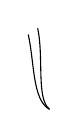
\begin{tikzpicture}[x=1cm,y=1cm]
\draw (0,0.95) .. controls (0.08,0.6) and (0.05,0.12) .. (0.27,0);
\draw (0.12,1.03) .. controls (0.2,0.65) and (0.1,0.14) .. (0.27,0);
\end{tikzpicture}}}\normalmarginpar pour les mém\unsure{\deleted{p}o|\deleted{o}p|p}ires de Segal quand tu les auras ; pense seulement à me dire combien cela fait de pages dactylographiées .

Meilleures amitiés\\
\handwritten{J A Dieudonné}\\
% archive sheet number: 95

\scanpage{97}
\handwritten{15.9.67.}\\

Cher Dieudonné,\\

Tes objections de ta lettre du 11 Septembre sont encore fondées. D'ailleurs, il ne me semble pas évident que le fait de pouvoir trouver $p,q$ fixes tels qu'on ait des suites exactes $A_n^p\quad A_n^q\quad M_n\quad0$, permette de s'en tirer; tant mieux si tu y arrives. L'existence de ces $p$ et $q$ me semble d'autre part facile, en utlisant le

\uline{Lemme}\quad Soit $A$ un anneau, $M$ un $A$-module, $(f_i)_{1\;i\;n}$ des éléments de $A$ engendrant l'idéal unité, \deleted{$m$ un entier} supposons que pour tout $i$, le $A_{f_i}$-module $M_{f_i}$ soit engendré par $m_i$ générateurs. Alors $M$ est engendré par $m\quad m_i$ générateurs.

Démonstration: soient $g_j^i\quad M_{f_i}\quad\unsure{(}1\quad j\quad m_i)$ les générateurs de $M_{f_i}$ , on aura donc $g_j^i=h_j^i/f_i^{N_{ij}}$ , avec $h_j^i\quad \unsure{\deleted{A}M|\deleted{M}A}$ . Alors les $\unsure{\deleted{g}h_j^i|\deleted{h}g_j^i}$ pour $j$ fixes engendrent $\overset{\handwritten{\sim}}{M}$ sur l'ouvert $\operatorname{Spec}(A_{f_i})$ de $\operatorname{Spec}(A_f)$, donc comme pour $i$ varaible ces ouverts recouvrent $\operatorname{Spec}(A)$, \unsure{\deleted{n}i|\deleted{o}i|\deleted{h}i|\deleted{i}n|\deleted{i}o|\deleted{i}h}l s'ensuit que les $h_j^i$ pour $i,j$ variables engendrent $\overset{\handwritten{\unsure{\sim}}}{M}$, donc $M$, ce qui établit le lemme.

Revenant alors à la situation de 10.10.5 , on sait que $M=\lim M_n$ est un $A$-module de type fini, considérons alors un ép\unsure{\deleted{m}i|\deleted{t}i|\deleted{i}m|\deleted{i}t}morphisme $u:A^q\quad M$ . Soient $f_i\quad A$ dont les images dans $A_o$ engendrent l'idéal unité, et tel que sur les \deleted{Spef(} ouverts correspondants $X_i$ de $X=\operatorname{Specf}(A)$, $F$ admette une présentation finie, donc soit de la forme $M_i$ , où $M_i$ est un $\inserted{A_i=}A_{f_i}$-\unsure{\deleted{ù}m|\deleted{à}m|\deleted{m}ù|\deleted{m}à}odul\unsure{e} de présentation finie. Alors $u$ restreint à $X_i$ définit un épimorphisme $A_i^q\quad M_i$ , et comme $M_i$ est de présentation finie, il existe un homomorphi\unsure{s}me $v_i$ rendant exacte la suite $A_i^p\quad A_i^q\quad M_i\quad0$ . Tensorisant par $A_o$ , on en déduit une suite exacte $(A_n)_{f_i}^p\quad(A_n)_{f_i}^q\quad(M_n)_{f_i}\quad0$, ce qui montre que,\deleted{le} si $R_n=\operatorname{Ker}(A_n^q\quad M_n)$, alors $R_n$ est sur $\operatorname{Spec}(A_{n\;f_i})$ engendré par $p$ éléments. Donc en vertu du lemme $R_n$ est engendré par $mp$ éléments
% archive sheet number: 96

\scanpage{98}
où $m$ est le nombre des $f_i$ , et $mp$ est bien indépendant de $n$.

La difficulté qui \deleted{reste} semble rester est de trouver les suites exactes que tu demandes de telle façon qu'elles se recollent, pour $n$ variable. Donc, $u$ étant déjà choisi, de trouver un homomorphisme $A^p\quad A^q$ \deleted{donnant $\unsure{u|n}$} dont l'image soit $\operatorname{Ker}u$ ... Si tu y arrives, on pourrait présenter encore 10.10.5 sous forme de trois conditions équivalentes, mais en demandant dans b) une ``prsentation finie\deleted{''} uniformément en $n$'' . Sinon, il faudrait trouver un contre-exemple à \deleted{l'équiva} l'implication a)\quad c) , car il me semble que la question devrait être tirée au clair. En tout état de cause, il faudra donner,en corollaire,l'équivalence des conditions suivantes, valables sans hypothèses noethériennes:

a) $F$ est localement libre de type fini.

b) $F$ est i\unsure{\deleted{i}s|\deleted{s}i}omorphe à la limite projective d'une suite $(F_n)$ de $\unsure{\text{\uuline{$O$}}|\text{\uline{$O$}}}_{X_n}$-Modules loc libres de type fini qui se recollent.

c) $F$ est isomorphe à un $M$ , avec $M$ un $A$-module projectif de type fini.

Pour la démonstration, on procède comme dans 10.10.5 en ut\uline{i}lisant EGA IV 18.3.2.1 . Ce lemme devrait d'ailleurs venir en corollaire \deleted{\unsure{7.|à|0}} après $\unsure{0|O}_I$ 7.2.9.

Pour les modifications que je préconaisais pour I 10.11 , elles tombent à l'eau s\unsure{\deleted{o}i|\deleted{i}o} on n'arrive pas à arranger 10.10.5 sans hypothèses noethériennes; on peut cependant dire que si $F$ sur $X$ est de présentation finie, alors il est limite projective de faisceaux $F_n$ de présentation finie sur les $X_n$ qui se recollent (mais on n'a pas une réciproque), et que $F$ est localement libre s\unsure{\deleted{s}i|\deleted{i}s}s les $F_n$ le sont. \unsure{\deleted{\unsure{S}}E|\deleted{E}\unsure{S}}t \deleted{10.11.4} les autres énoncés du n\unsure{0|\deleted{0}°|\deleted{°}0|°} 10.11. restent valables\unsure{\deleted{,}|x} sans hypothèse noe\unsure{\deleted{h}t|\deleted{t}h}hérienne, sauf 10.7.11.2 et la partie ``injectivité'' dans 10.11.9 (sauf erreur).
% archive sheet number: 97
